The Explorer and Knowledge Flow environments help you determine how
well machine learning schemes perform on given datasets. But serious
investigative work involves substantial experiments---typically
running several learning schemes on different datasets, often with
various parameter settings---and these interfaces are not really
suitable for this. The Experimenter enables you to set up large-scale
experiments, start them running, leave them, and come back when they
have finished and analyze the performance statistics that have been
collected. They automate the experimental process. The statistics can
be stored in ARFF format, and can themselves be the subject of further
data mining. You invoke this interface by selecting
\textit{Experimenter} from the choices at the side of the panel in
Figure~\ref{subfig:explorer_1}.

Whereas the Knowledge Flow transcends limitations of space by allowing
machine learning runs that do not load in the whole dataset at once,
the Experimenter transcends limitations of time. It contains
facilities for advanced users to distribute the computing load across
multiple machines using Java RMI. You can set up big experiments and
just leave them to run.

\section{Getting started}

\begin{lrbox}{\verbbox}
\begin{minipage}{.98\textwidth}
\begin{mdframed}[innermargin=-1.5cm]
\begin{Verbatim}[fontsize=\scriptsize]
Key_Dataset,Key_Run,Key_Fold,Key_Scheme,Key_Scheme_options,Key_Scheme_version_ID,Date_time,
Number_of_training_instances,Number_of_testing_instances,Number_correct,Number_incorrect,
Number_unclassified,Percent_correct,Percent_incorrect,Percent_unclassified,Kappa_statistic,
Mean_absolute_error,Root_mean_squared_error,Relative_absolute_error,Root_relative_squared_error,
SF_prior_entropy,SF_scheme_entropy,SF_entropy_gain,SF_mean_prior_entropy,SF_mean_scheme_entropy,
SF_mean_entropy_gain,KB_information,KB_mean_information,KB_relative_information,True_positive_rate,
Num_true_positives,False_positive_rate,Num_false_positives,True_negative_rate,Num_true_negatives,
False_negative_rate,Num_false_negatives,IR_precision,IR_recall,F_measure,Matthews_correlation,
Area_under_ROC,Area_under_PRC,Weighted_avg_true_positive_rate,Weighted_avg_false_positive_rate,
Weighted_avg_true_negative_rate,Weighted_avg_false_negative_rate,Weighted_avg_IR_precision,
Weighted_avg_IR_recall,Weighted_avg_F_measure,Weighted_avg_matthews_correlation,
Weighted_avg_area_under_ROC,Weighted_avg_area_under_PRC,Unweighted_macro_avg_F_measure,
Unweighted_micro_avg_F_measure,Elapsed_Time_training,Elapsed_Time_testing,UserCPU_Time_training,
UserCPU_Time_testing,UserCPU_Time_millis_training,UserCPU_Time_millis_testing,Serialized_Model_Size,
Serialized_Train_Set_Size,Serialized_Test_Set_Size,Coverage_of_Test_Cases_By_Regions,
Size_of_Predicted_Regions,Summary,measureTreeSize,measureNumLeaves,measureNumRules
iris,1,1,weka.classifiers.trees.J48,'-C 0.25 -M 2',-217733168393644444,2.01604080413E7,135.0,15.0,
14.0,1.0,0.0,93.33333333333333,6.666666666666667,0.0,0.9,0.0450160137965016,0.1693176548766098,
10.128603104212857,35.917698581356284,23.77443751081735,2.632715099281766,21.141722411535582,
1.5849625007211567,0.17551433995211774,1.4094481607690388,21.615653599867994,1.4410435733245328,
1363.79589990507,1.0,5.0,0.0,0.0,1.0,10.0,0.0,0.0,1.0,1.0,1.0,1.0,1.0,1.0,0.9333333333333333,
0.03333333333333333,0.9666666666666667,0.06666666666666667,0.9444444444444445,0.9333333333333333,
0.9326599326599326,0.9062760897356267,1.0,1.0,0.9326599326599326,0.9333333333333333,0.008,0.001,
0.0062889999999999995,5.809999999999999E-4,6.289,0.581,4236.0,10633.0,2353.0,100.0,35.55555555555555,
'Number of leaves: 4\nSize of the tree: 7\n',7.0,4.0,4.0
\end{Verbatim}
\end{mdframed}
\end{minipage}
\end{lrbox}%

\begin{figure}[!p]
\centering
\subfloat[Setting it up.]{\label{subfig:experimenter_1}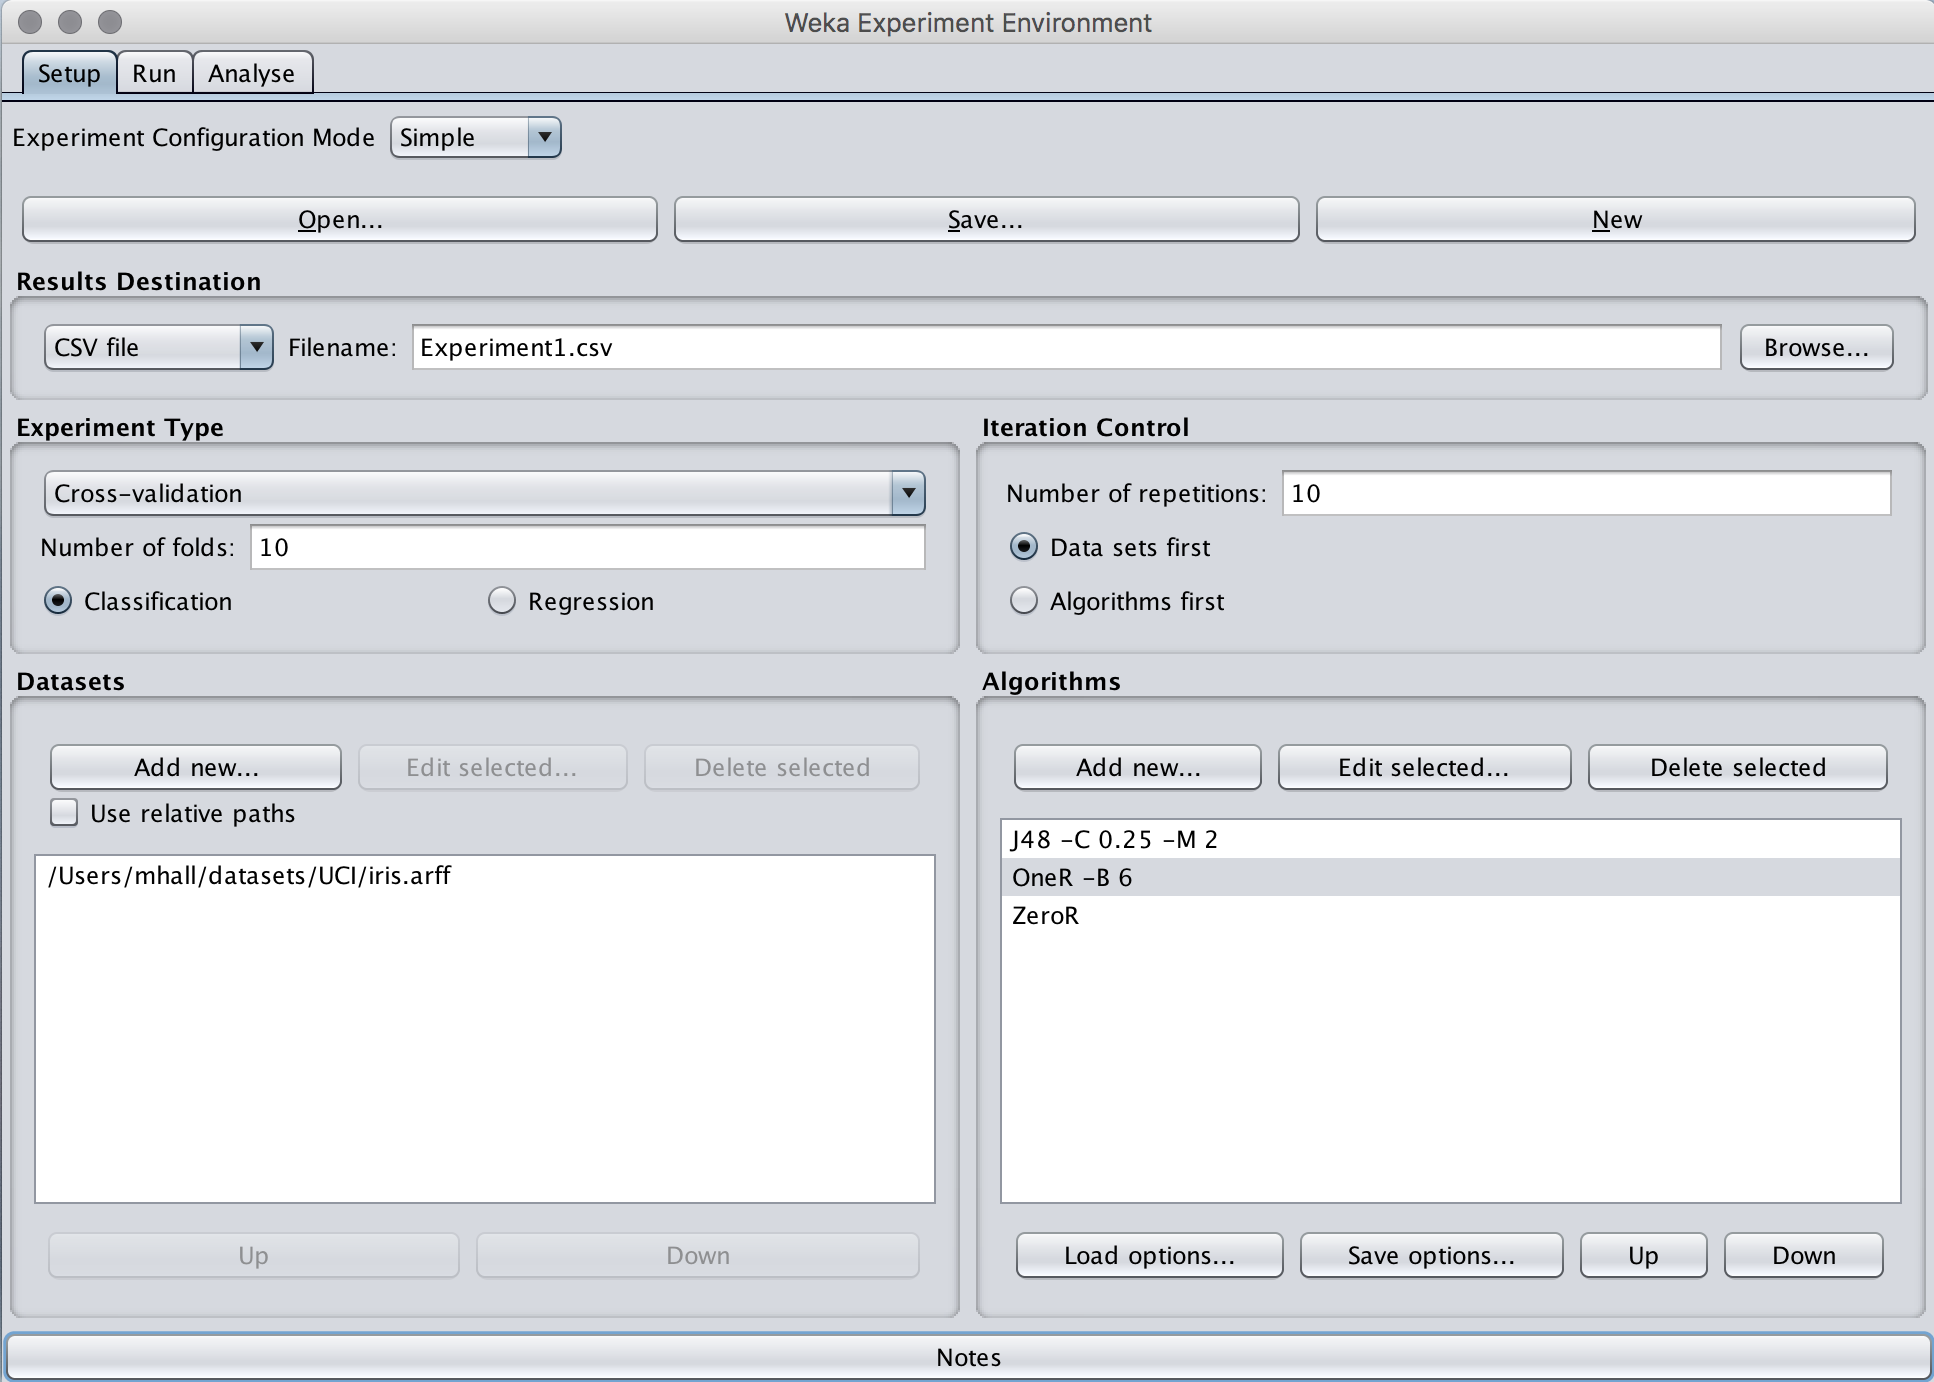
\includegraphics[width=0.95\textwidth]{images/B4_1a.png}}
\newline
\subfloat[The results file.]{\label{subfig:experimenter_2} \usebox{\verbbox}}
\newline
\subfloat[Spreadsheet with results.]{\label{subfig:experimenter_3}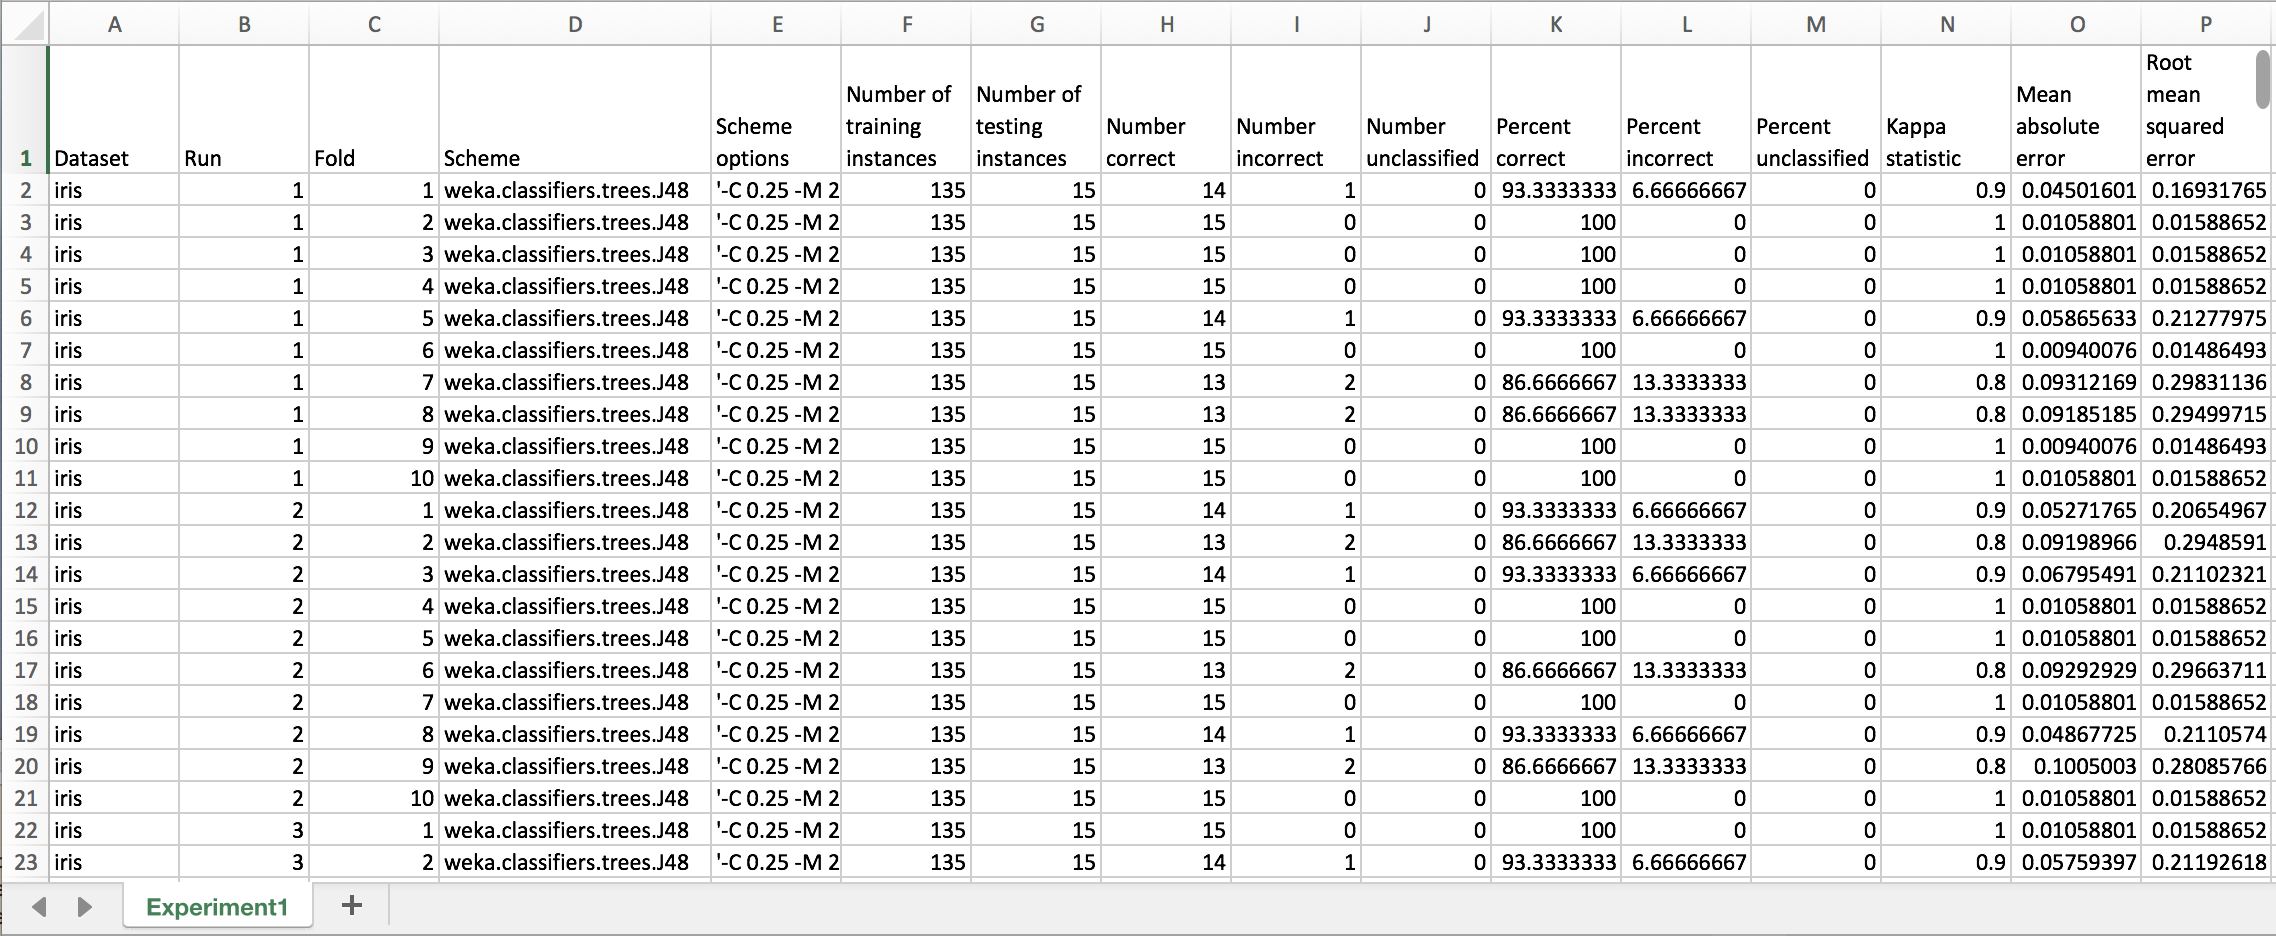
\includegraphics[width=0.95\textwidth]{images/B4_1c.png}}
\caption{\label{fig:experimenter}A experiment.}
\end{figure}

As an example, we will compare the J4.8 decision tree method with the
baseline methods \textit{OneR} and \textit{ZeroR} on the iris
dataset. The Experimenter has three panels: \textit{Setup},
\textit{Run} and \textit{Analyze}. Figure~\ref{subfig:experimenter_1}
shows the first: you select the others from the tabs at the top. Here,
the experiment has already been set up. To do this, first click New
(toward the right at the top) to start a new experiment (the other two
buttons in that row save an experiment and open a previously saved
one). Then, on the line below, select the destination for the
results---in this case the file \textit{Experiment1}---and choose
\textit{CSV file}. Underneath, select the datasets---we have only one,
the iris data. To the right of the datasets, select the algorithms to
be tested---we have three. Click \textit{Add} new to get a standard
Weka object editor from which you can choose and configure a
classifier. Repeat this operation to add the three classifiers. Now
the experiment is ready.

The other settings in Figure~\ref{subfig:experimenter_1} are all
default values. If you want to reconfigure a classifier that is already
in the list, you can use the \textit{Edit selected} button. You can
also save the options for a particular classifier in XML format for
later reuse. You can right-click on an entry to copy the configuration
to the clipboard, and add or enter a configuration from the clipboard.

\section{Running an experiment}

To run the experiment, click the \textit{Run} tab, which brings up a
panel that contains a \textit{Start} button (and little else); click
it. A brief report is displayed when the operation is finished. The
file \textit{Experiment1.csv} contains the results. The first two
lines are shown in Figure~\ref{subfig:experimenter_2}: they are in CSV
format and can be read directly into a spreadsheet, the first part of
which appears in Figure~\ref{subfig:experimenter_3}. Each row
represents 1 fold of a 10-fold cross-validation (see the \textit{Fold}
column). The cross-validation is run 10 times (the \textit{Run}
column) for each classifier (the \textit{Scheme} column). Thus the
file contains 100 rows for each classifier, which makes 300 rows in
all (plus the header row). Each row contains plenty of information,
including the options supplied to the machine learning scheme; the
number of training and test instances; the number (and percentage) of
correct, incorrect, and unclassified instances; the mean absolute
error, root mean-squared error, and many more.

There is a great deal of information in the spreadsheet, but it is
hard to digest. In particular, it is not easy to answer the question
posed previously: how does J4.8 compare with the baseline methods
\textit{OneR} and \textit{ZeroR} on this dataset? For that we need the
\textit{Analyze} panel.

\section{Analyzing the results}

The reason that we generated the output in CSV format was to show the
spreadsheet in Figure~\ref{subfig:experimenter_3}. The Experimenter
normally produces its output in ARFF format. You can also leave the
file name blank, in which case the Experimenter stores the results in
a temporary file.

\begin{figure}[!th]
\centering
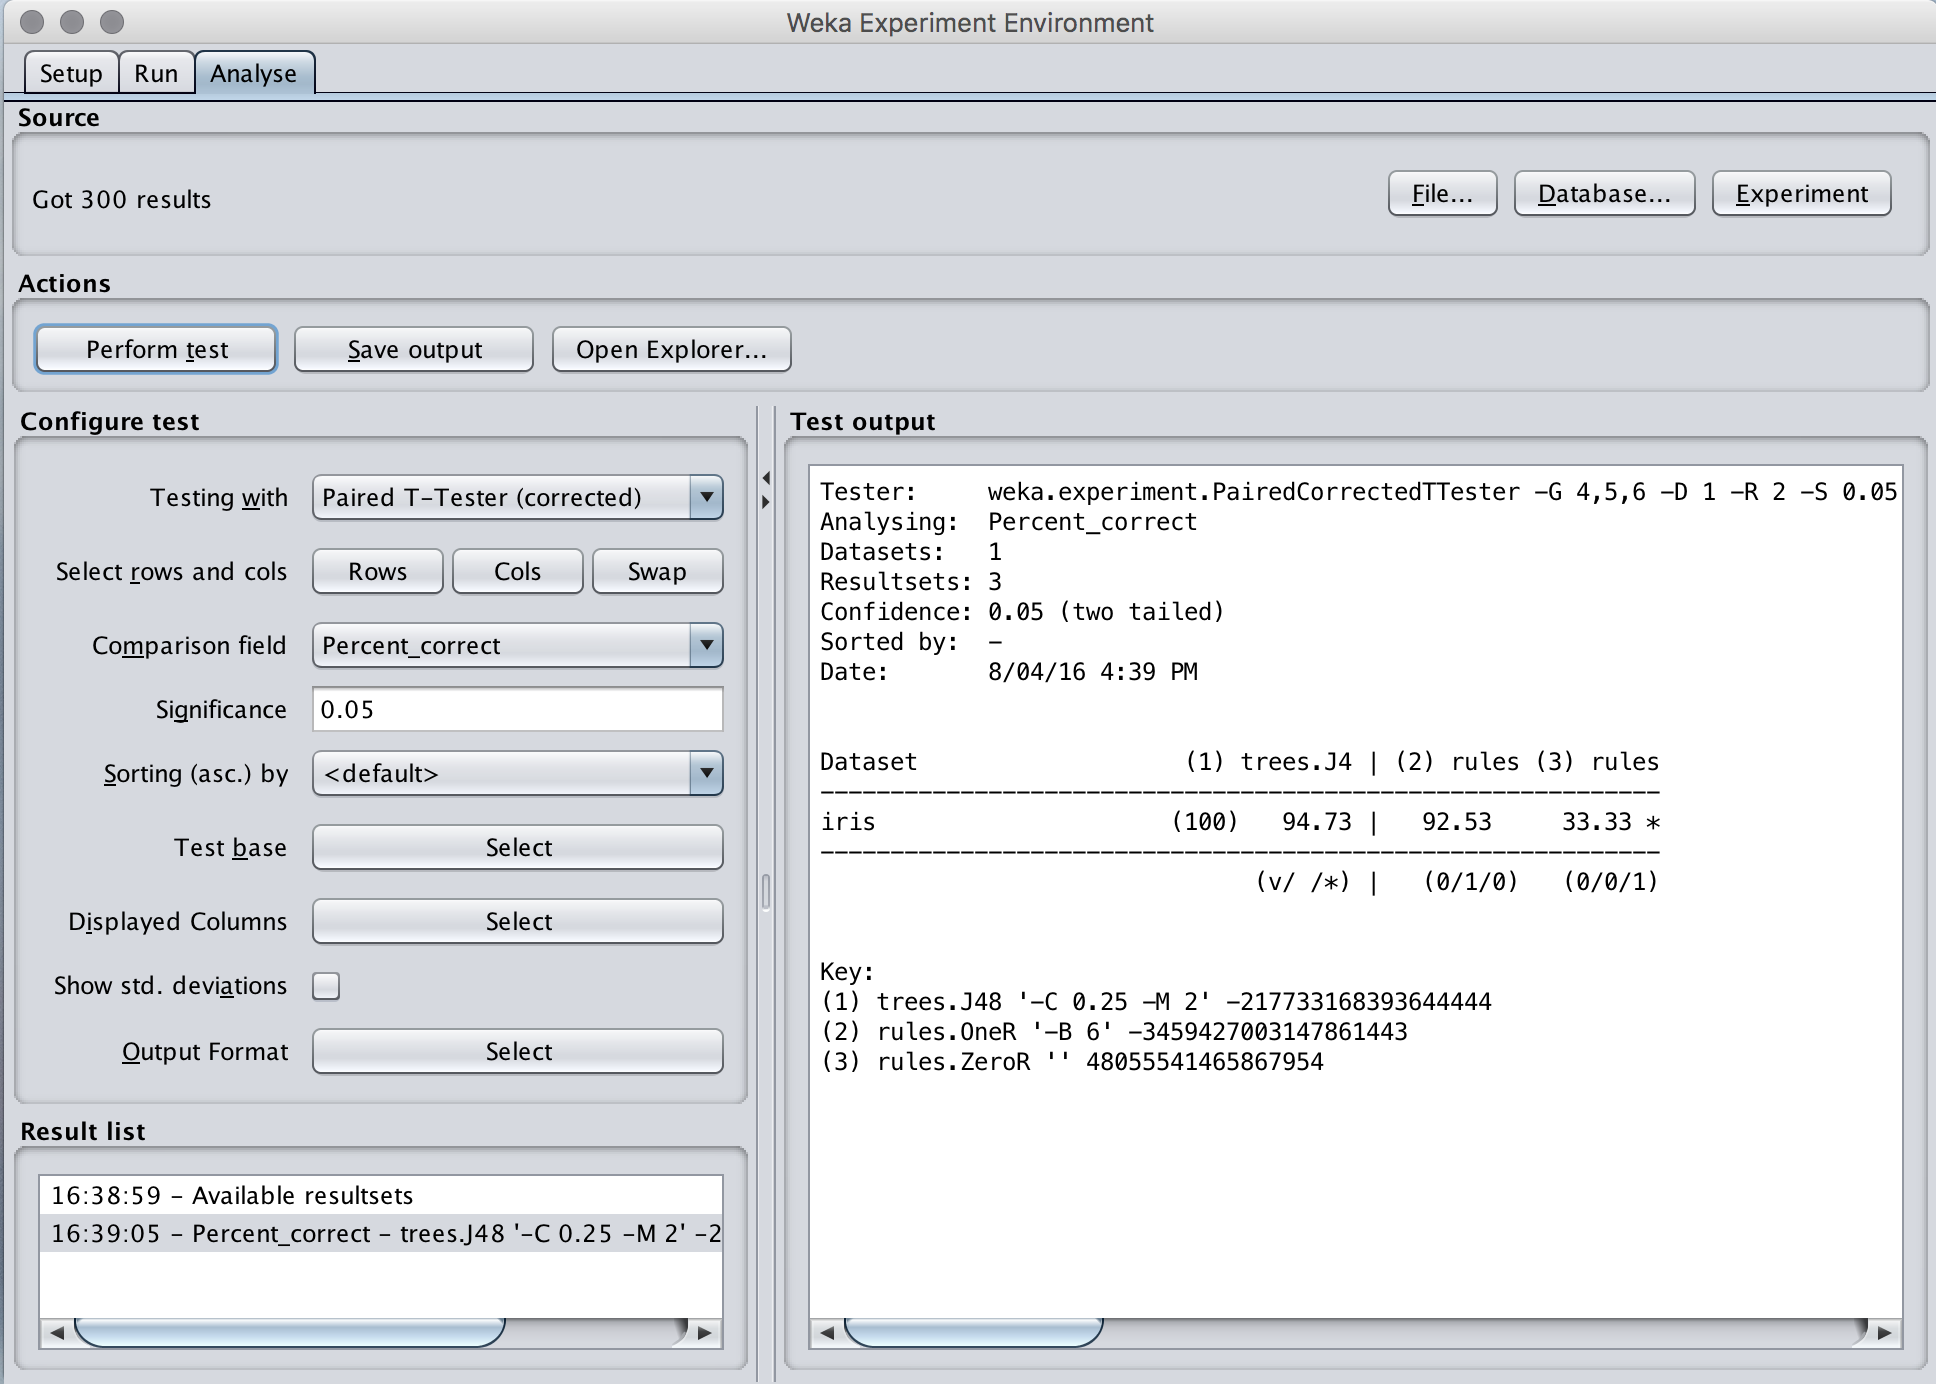
\includegraphics[width=0.95\textwidth]{images/B4_2.png}
\caption{Statistical test results for the experiment of Figure~\ref{subfig:experimenter_1}.}
\label{fig:experimenter_analyze}
\end{figure}

The \textit{Analyze} panel is shown in
Figure~\ref{fig:experimenter_analyze}. To analyze the experiment that
has just been performed, click the \textit{Experiment} button at the
right near the top; otherwise, supply a file that contains the results
of another experiment. Then click \textit{Perform test} (near the
bottom on the left). The result of a statistical significance test of
the performance of the first learning scheme (\textit{J48}) versus the
other two (\textit{OneR} and \textit{ZeroR}) will be displayed in the
large panel on the right.

We are comparing the percent correct statistic: this is selected by
default as the comparison field shown toward the left of
Figure~\ref{fig:experimenter_analyze}. The three methods are displayed
horizontally, numbered \textit{(1)}, \textit{(2)}, and \textit{(3)},
as the heading of a little table. The labels for the columns are
repeated at the bottom---\textit{trees.J48}, \textit{rules.OneR}, and
\textit{rules.ZeroR}---in case there is insufficient space for them in
the heading. The inscrutable integers beside the scheme names identify
which version of the scheme is being used. They are present by default
to avoid confusion among results generated using different versions of
the algorithms. The value in brackets at the beginning of the iris row
\textit{(100)} is the number of experimental runs: 10 times 10-fold
cross-validation.

The percentage correct for the three schemes is shown in
Figure~\ref{fig:experimenter_analyze} 94.73\% for method 1, 92.53\%
for method 2, and 33.33\% for method 3. The symbol placed beside a
result indicates that it is statistically better ($v$) or worse (*)
than the baseline scheme---in this case J4.8---at the specified
significance level (0.05, or 5\%). The corrected resampled $t$-test is
used here. Here, method 3 is significantly worse than method 1,
because its success rate is followed by an asterisk. At the bottom of
columns 2 and 3 are counts (x/y/z) of the number of times the scheme
was better than (x), the same as (y), or worse than (z) the baseline
scheme on the datasets used in the experiment. In this case there is
only one dataset; method 2 was equivalent to method 1 (the baseline)
once, and method 3 was worse than it once. (The annotation ($v$/  /*) is
placed at the bottom of column 1 to help you remember the meanings of
the three counts x/y/z.)

\section{Simple setup}

In the \textit{Setup} panel of Figure~\ref{subfig:experimenter_1} we
left most options at their default values. The experiment type is a
10-fold cross-validation repeated 10 times. You can alter the number
of folds in the box at center left and the number of repetitions in
the box at center right. The experiment type is classification; you
can specify regression instead. You can choose several datasets, in
which case each algorithm is applied to each dataset, and change the
order of iteration using the \textit{Data sets first} and
\textit{Algorithm first} buttons. The alternative to cross-validation
is the holdout method. There are two variants, depending on whether
the order of the dataset is preserved or the data is randomized. You
can specify the percentage split (the default is two-thirds training
set and one-third test set).

Experimental setups can be saved and reopened. You can make notes
about the setup by pressing the \textit{Notes button}, which brings up
an editor window. Serious Weka users soon find the need to open up an
experiment and rerun it with some modifications---perhaps with a new
dataset or a new learning algorithm. It would be nice to avoid having
to recalculate all the results that have already been obtained! If the
results have been placed in a database rather than an ARFF or CSV
file, this is exactly what happens. You can choose \textit{JDBC
  database} in the results destination selector and connect to any
database that has a JDBC driver. You need to specify the database’s
URL and enter a username and password. To make this work with your
database you may need to modify the
\textit{weka/experiment/DatabaseUtils.props} file in the Weka
distribution. If you alter an experiment that uses a database, Weka
will reuse previously computed results whenever they are
available. This greatly simplifies the kind of iterative
experimentation that typically characterizes data mining research.

\section{Advanced setup}

\begin{figure}[!th]
\centering
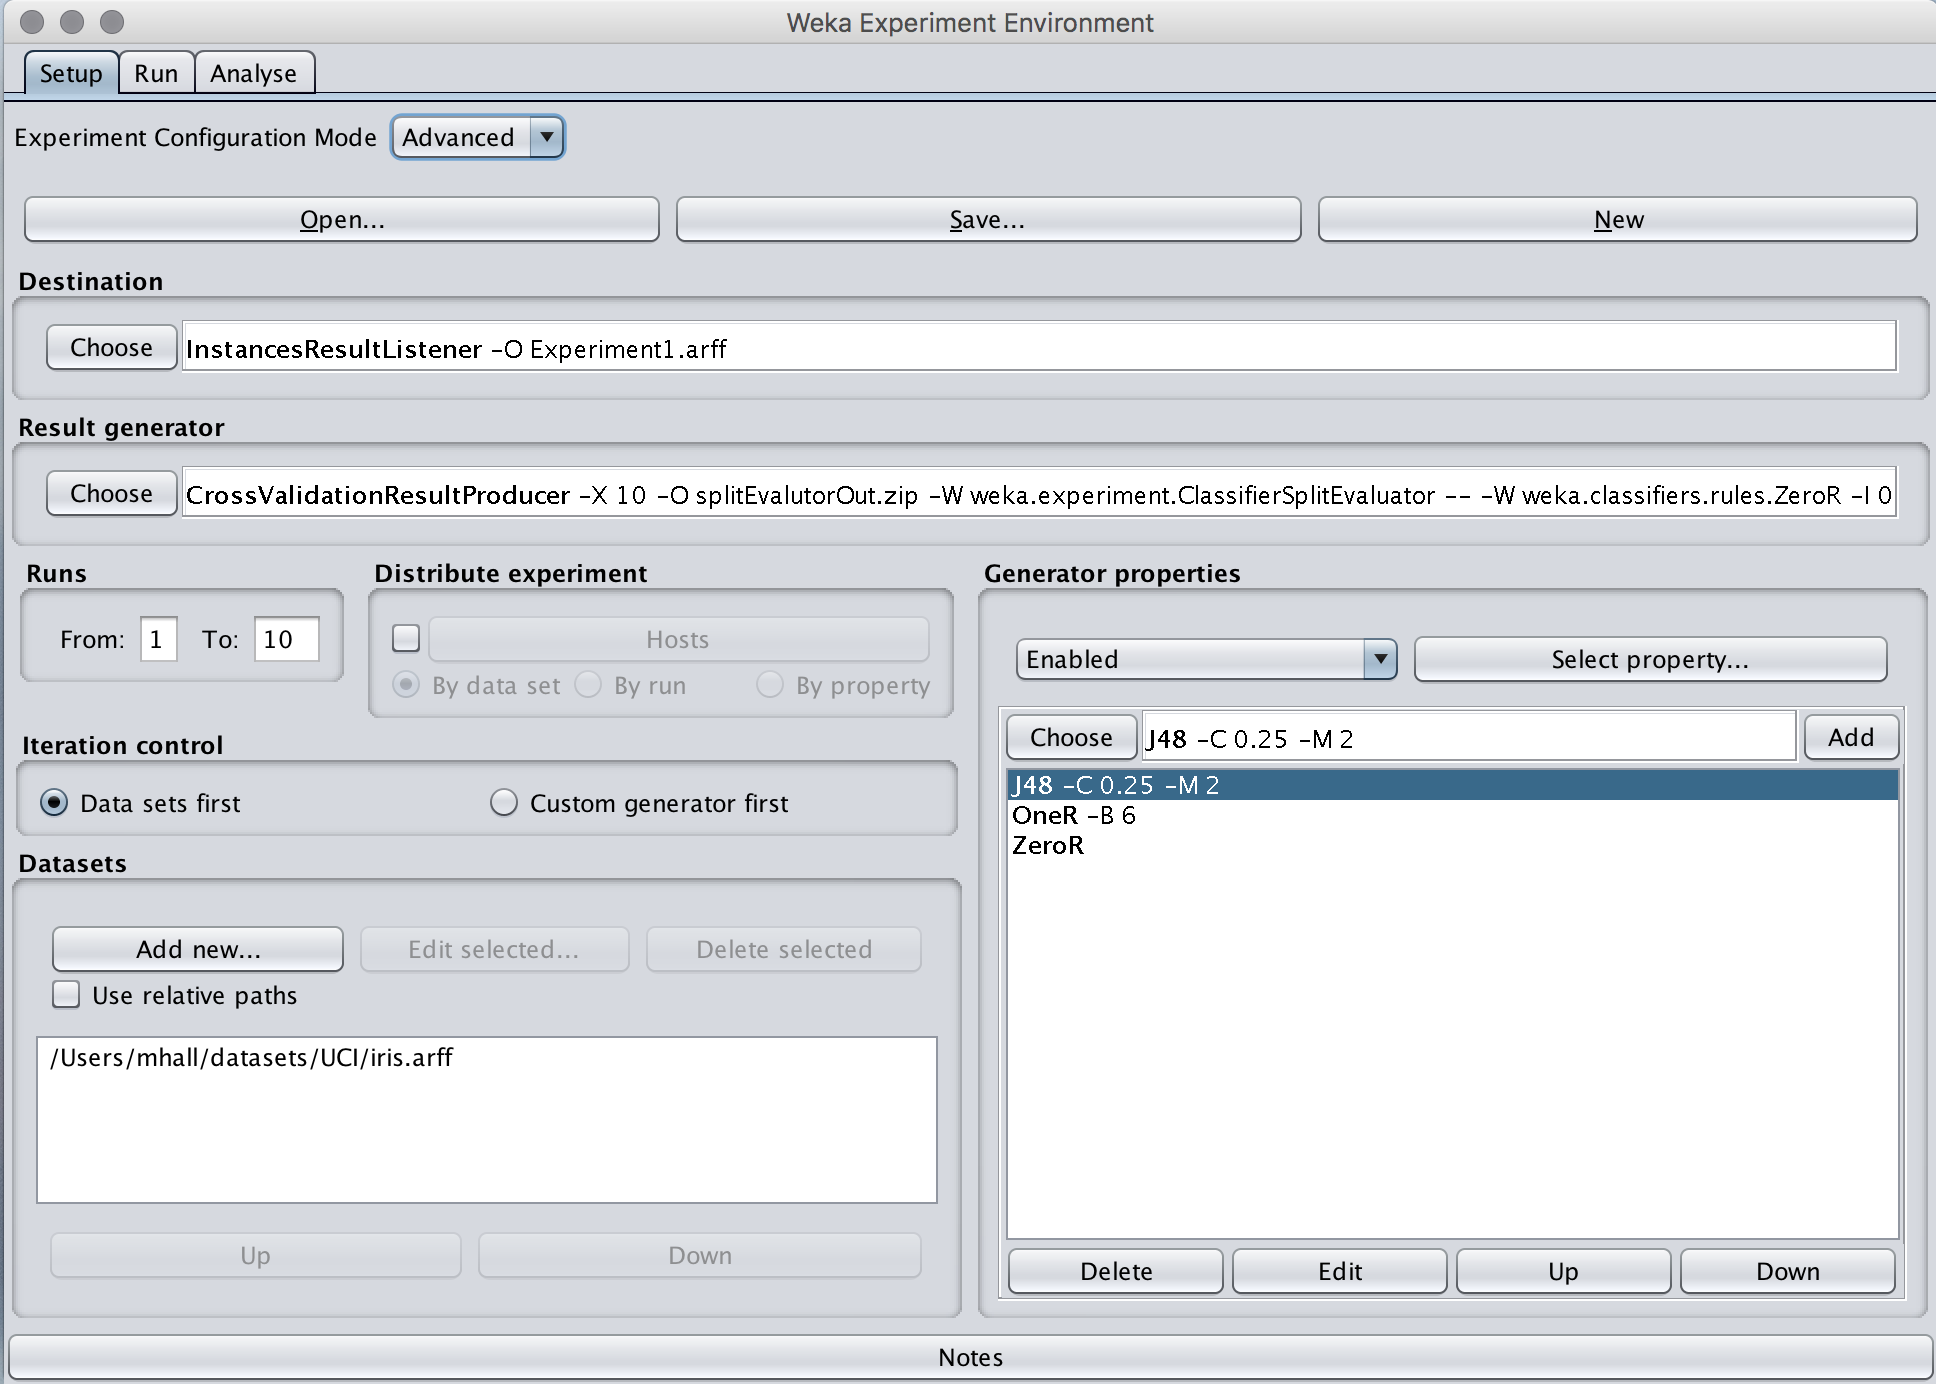
\includegraphics[width=0.95\textwidth]{images/B4_3.png}
\caption{Setting up an experimenter in advanced mode.}
\label{fig:experimenter_advanced}
\end{figure}


The Experimenter has an advanced mode. Select \textit{Advanced} from
the drop down box near the top of the panel shown in
Figure~\ref{subfig:experimenter_1} to obtain the more formidable
version of the panel shown in
Figure~\ref{fig:experimenter_advanced}. This enlarges the options
available for controlling the experiment---including, for example, the
ability to generate learning curves. However, the advanced mode is
hard to use, and the simple version suffices for most purposes. For
example, in advanced mode you can set up an iteration to test an
algorithm with a succession of different parameter values, but the
same effect can be achieved in simple mode by putting the algorithm
into the list several times with different parameter values.

\begin{figure}[!thp]
\centering
\subfloat[Generator properties.]{\label{subfig:experimenter_cluster_1}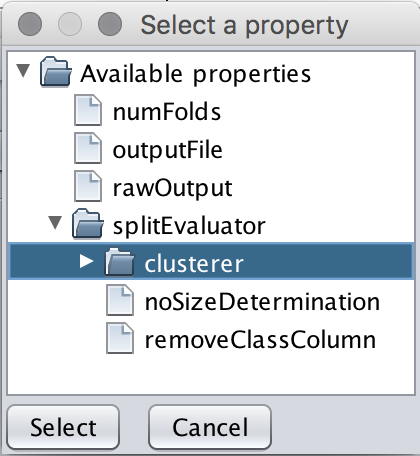
\includegraphics[width=0.2\textwidth]{images/B4_4a.png}}
\qquad
\subfloat[Two clustering schemes.]{\label{subfig:experimenter_cluster_2}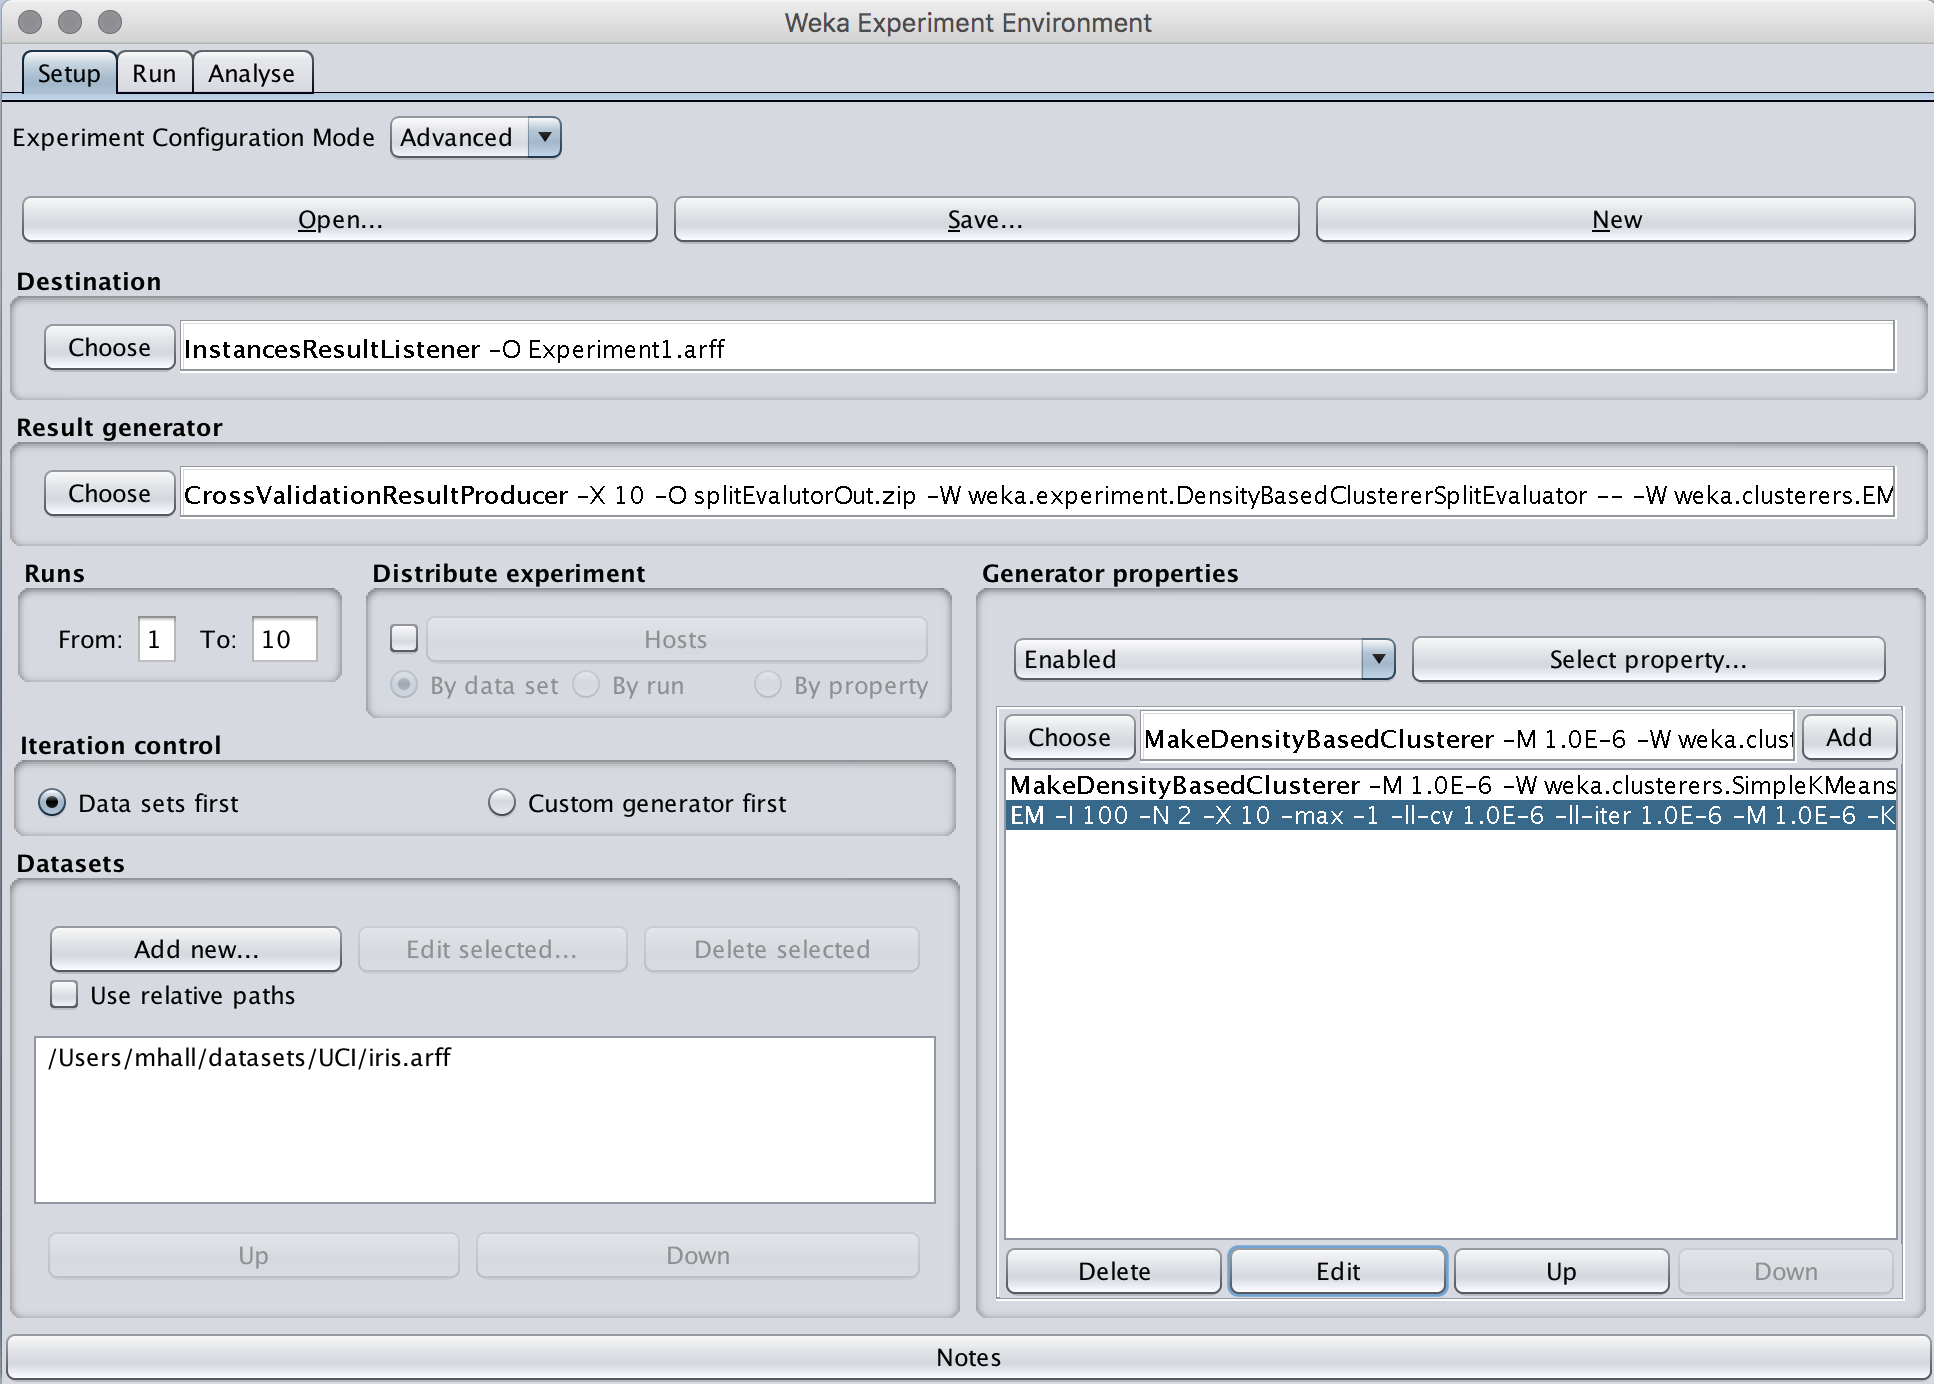
\includegraphics[width=0.7\textwidth]{images/B4_4b.png}}
\newline
\subfloat[Analyze panel.]{\label{subfig:experimenter_cluster_3}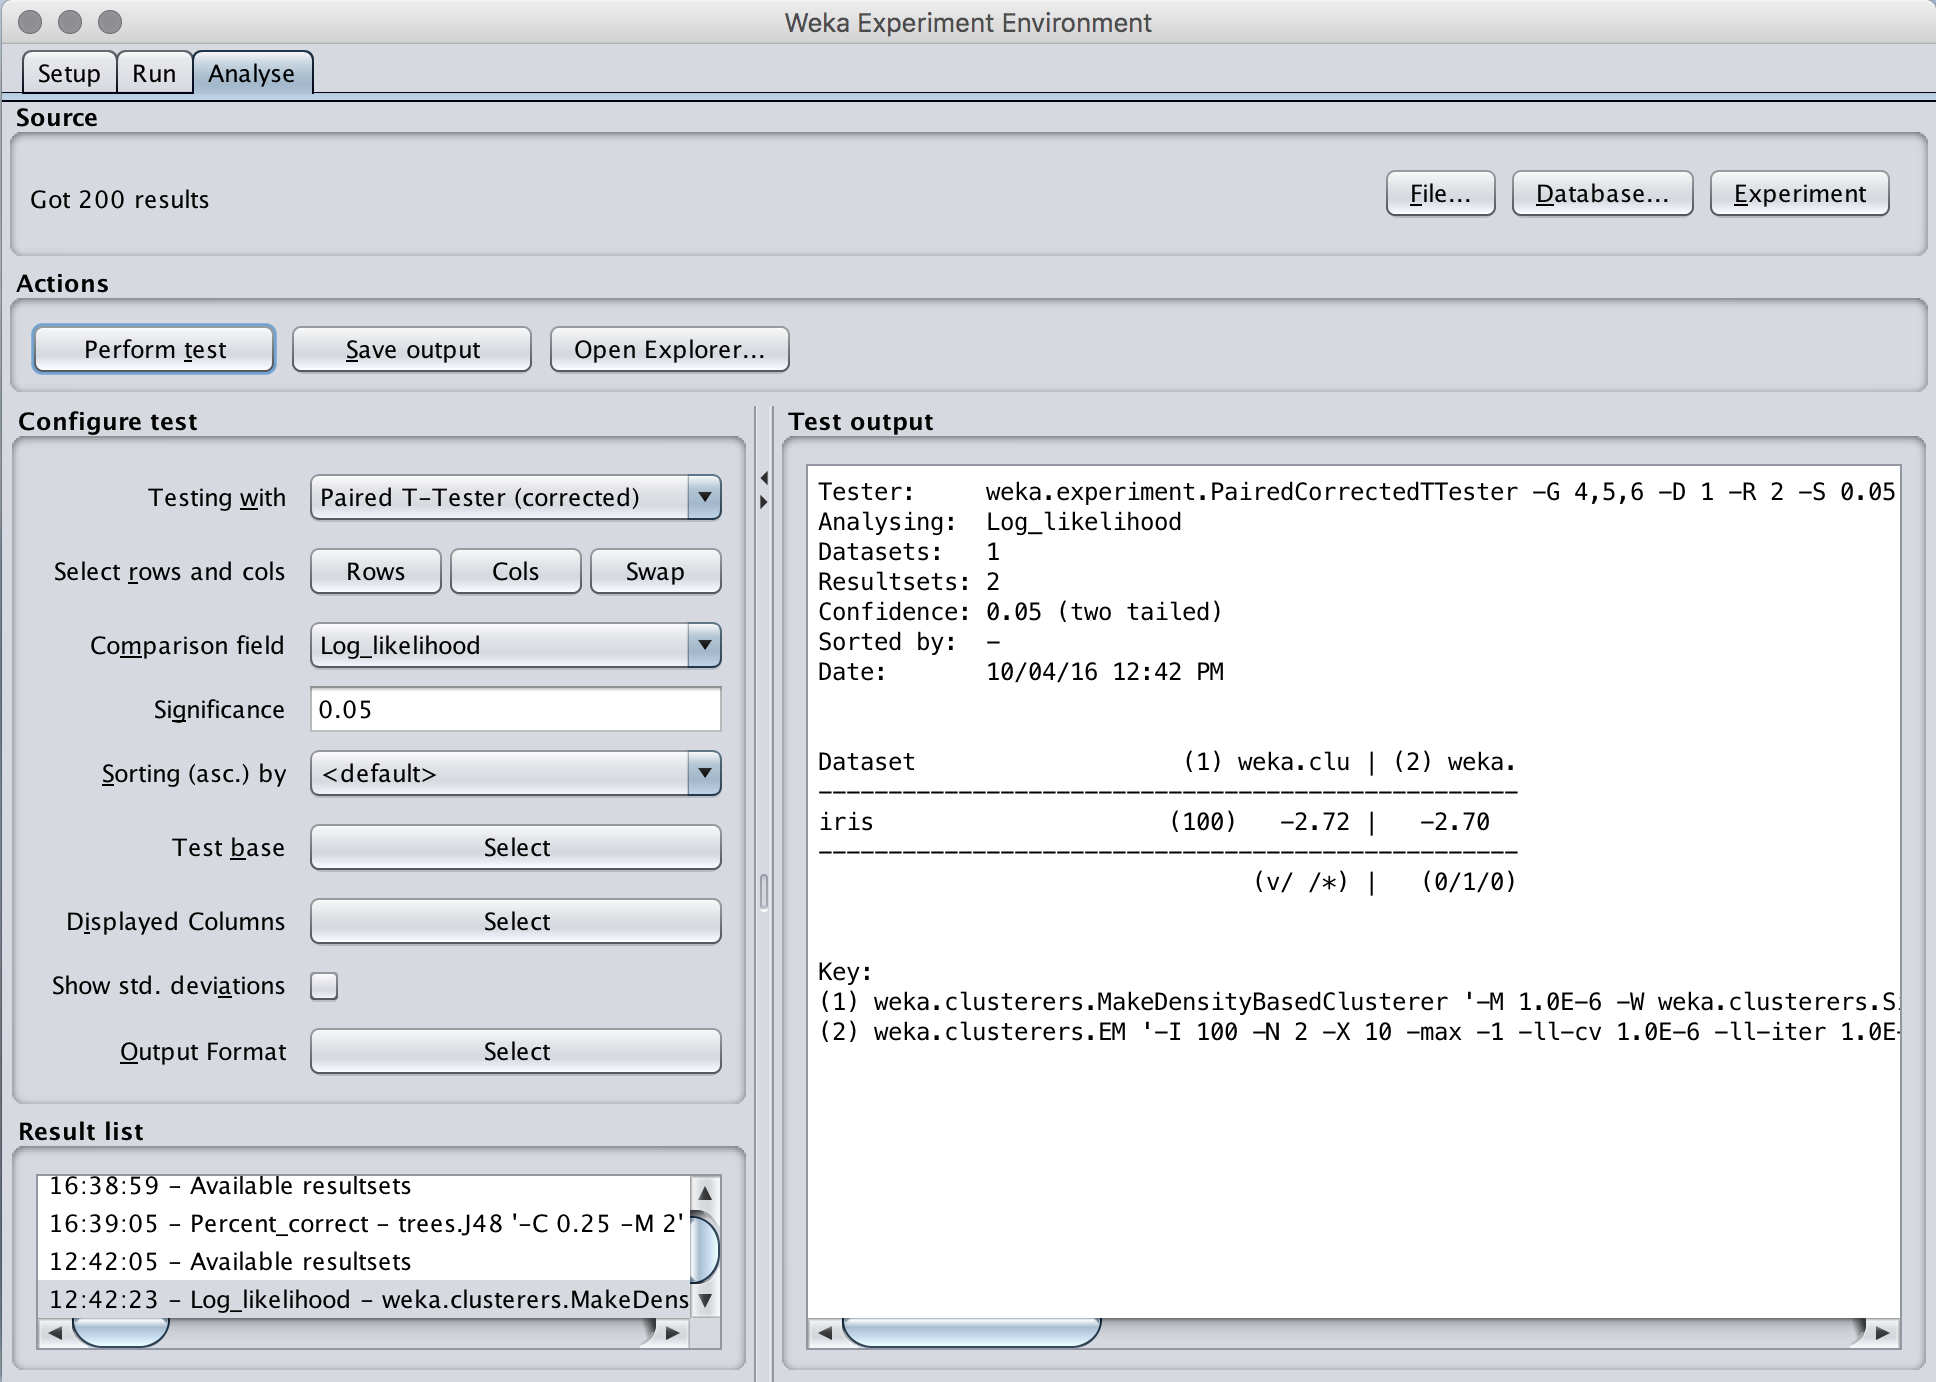
\includegraphics[width=0.8\textwidth]{images/B4_4c.png}}
\caption{\label{fig:experimenter_cluster}An experiment in clustering.}
\end{figure}

One thing you can do in advanced mode but not in simple mode is run
experiments using clustering algorithms. Here, experiments are limited
to those clusterers that can compute probability or density estimates,
and the main evaluation measure for comparison purposes is the log
likelihood. To set this up quickly, first click the \textit{Result
  generator} to bring up an object editor for the
\textit{CrossValidationResultProducer}. Then click the \textit{Choose}
button for the split evaluator and select
\textit{DensityBasedClustererSplitEvaluator} from the list. At this
point the panel on the lower right that contained the list of
classifiers goes blank and the \textit{Generator properties} drop-down
box displays \textit{Disabled}. Re-enable this, and a new window
appears with a list of properties
(Figure~\ref{subfig:experimenter_cluster_1}). Expand the
splitEvaluator entry, select clusterer (as shown in the Figure), and
click the Select button. Now the active list will reappear in the
bottom right-hand panel, along with the ability to add clustering
schemes, just as we did with classifiers.

Figure~\ref{subfig:experimenter_cluster_2} shows a setup with two
clustering schemes configured: \textit{EM} and the
\textit{MakeDensityBasedClusterer} wrapped around
\textit{SimpleKMeans}. After running this experiment, these two can be
compared in the \textit{Analyze} panel. The comparison field is not
set up with a meaningful default, so choose Log\_likelihood from the
drop-down box before pressing the \textit{Perform test}
button. Figure~\ref{subfig:experimenter_cluster_3} shows the results
for these clustering algorithms.

Another thing you may need the advanced mode for is to set up
distributed experiments, which we describe in
Section~\ref{section:experimenter_distributed}

\section{The Analyze panel}

Our walkthrough used the \textit{Analyze} panel to perform a
statistical significance test of one learning scheme (\textit{J48})
versus two others (\textit{OneR} and \textit{ZeroR}). The test was on
the error rate---the \textit{Comparison} field in
Figure~\ref{fig:experimenter_analyze}. Other statistics can be
selected from the drop-down menu instead: percentage incorrect,
percentage unclassified, root mean-squared error, the remaining error
measures from Table 5.8 (page 195), and various entropy
figures. Moreover, you can see the standard deviation of the attribute
being evaluated by ticking the \textit{Show std deviations} checkbox.

Use the \textit{Test base} menu to change the baseline scheme from
J4.8 to one of the other learning schemes. For example, selecting
\textit{OneR} causes the others to be compared with this scheme. In
fact, that would show that there is a statistically significant
difference between \textit{OneR} and \textit{ZeroR} but not between
\textit{OneR} and \textit{J48}. Apart from the learning schemes, there
are two other choices in the \textit{Select base} menu:
\textit{Summary} and \textit{Ranking}. The former compares each
learning scheme with every other scheme and prints a matrix whose
cells contain the number of datasets on which one is significantly
better than the other. The latter ranks the schemes according to the
total number of datasets that represent wins ($>$) and losses ($<$) and
prints a league table. The first column in the output gives the
difference between the number of wins and the number of losses.

\begin{figure}[!hp]
\centering
\subfloat[Row field.]{\label{subfig:experimenter_rows_and_cols_1}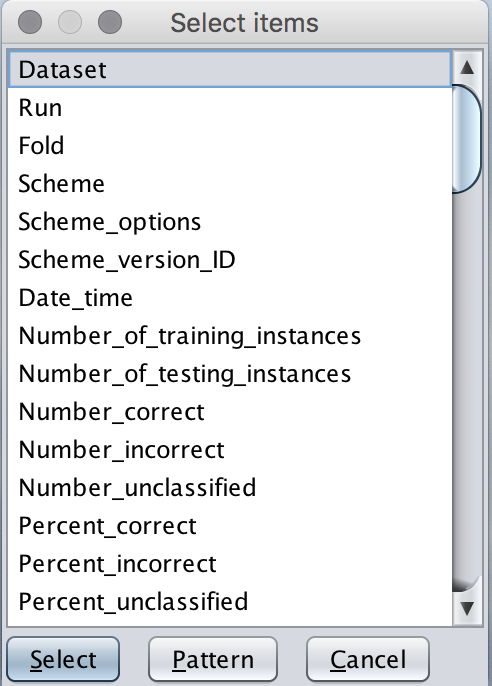
\includegraphics[width=0.45\textwidth]{images/B4_5a.png}}
\qquad
\subfloat[Column field.]{\label{subfig:experimenter_rows_and_cols_2}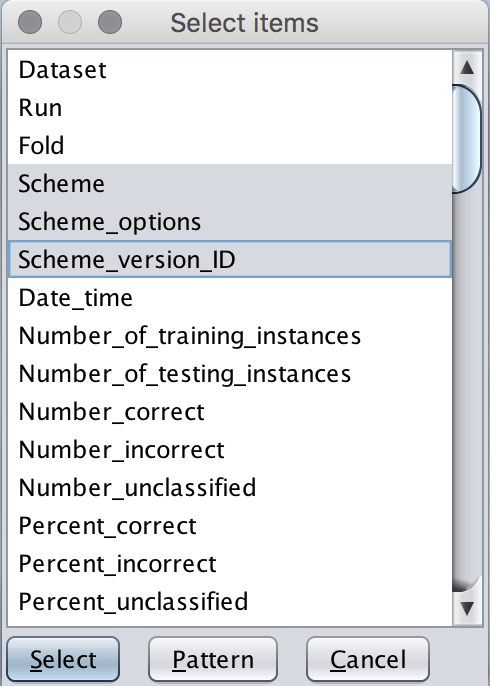
\includegraphics[width=0.45\textwidth]{images/B4_5b.png}}
\newline
\subfloat[Result of swapping the row and column selections.]{\label{subfig:experimenter_rows_and_cols_3}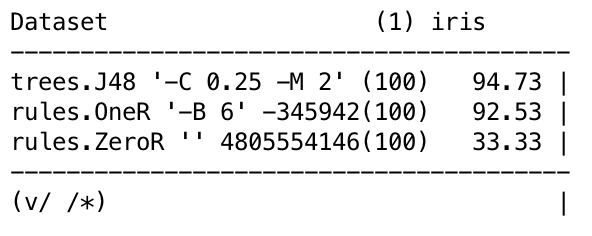
\includegraphics[width=0.45\textwidth]{images/B4_5c.png}}
\qquad
\subfloat[Substituting \textit{Run} for \textit{Dataset} as the rows.]{\label{subfig:experimenter_rows_and_cols_4}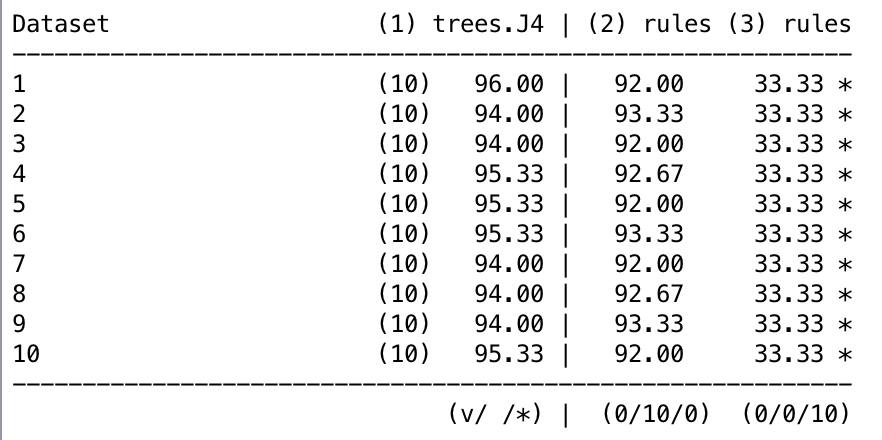
\includegraphics[width=0.45\textwidth]{images/B4_5d.png}}
\caption{\label{fig:experimenter_rows_and_cols}Rows and columns of Figure~\ref{fig:experimenter_analyze}.}
\end{figure}

The \textit{Row} and \textit{Column} fields determine the dimensions
of the comparison matrix. Clicking \textit{Select} brings up a list of
all the features that have been measured in the experiment---in other
words, the column labels of the spreadsheet in
Figure~\ref{subfig:experimenter_3}. You can select which to use as the
rows and columns of the matrix. (The selection does not appear in the
\textit{Select} box because more than one parameter can be chosen
simultaneously.) Figure~\ref{fig:experimenter_rows_and_cols} shows
which items are selected for the rows and columns of
Figure~\ref{fig:experimenter_analyze}. The two lists show the
experimental parameters (the columns of the spreadsheet). Dataset is
selected for the rows (and there is only one in this case, the iris
dataset), and \textit{Scheme}, \textit{Scheme options}, and
\textit{Scheme\_version\_ID} are selected for the column (the usual
convention of shift-clicking selects multiple entries). All three can
be seen in Figure~\ref{fig:experimenter_analyze}---in fact, they are
more easily legible in the key at the bottom.

If the row and column selections were swapped and the \textit{Perform
  test} button pressed again, the matrix would be transposed, giving
the result in Figure~\ref{fig:experimenter_rows_and_cols}. There
are now three rows, one for each algorithm, and one column, for the
single dataset. If instead the row of \textit{Dataset} were replaced
by \textit{Run} and the test were performed again, the result would be
as in Figure 4.5d. Run refers to the runs of the cross-validation, of
which there are 10, so there are now 10 rows. The number in
parentheses after each row label (100 in Figure 4.5c and 10 in Figure
4.5d) is the number of results corresponding to that row—in other
words, the number of measurements that participate in the averages
displayed by the cells in that row.

There is a button that allows you to select a subset of columns to
display (the baseline column is always included), and another that
allows you to select the output format: plain text (default), output
for the LaTeX typesetting system, CSV format, HTML, data and script
suitable for input to the GNUPlot graph plotting software, and just
the significance symbols in plain text format. It is also possible to
show averages and abbreviate filter class names in the output.

There is an option to choose whether to use the paired corrected
$t$-test or the standard $t$-test for computing significance. The way
the rows are sorted in the results table can be changed by choosing
the \textit{Sorting (asc.)} by option from the drop-down box. The
default is to use natural ordering, presenting them in the order that
the user entered the dataset names in the \textit{Setup}
panel. Alternatively the rows can be sorted according to any of the
measures that are available in the \textit{Comparison field}.

\section{Distributing processing over several machines}
\label{section:experimenter_distributed}

A remarkable feature of the Experimenter is that it can split up an
experiment and distribute it across several processors. This is for
advanced Weka users and is only available from the advanced version of
the \textit{Setup} panel. Some users avoid working with this panel by
setting the experiment up on the simple version and switching to the
advanced version to distribute it, because the experiment's structure
is preserved when you switch. However, distributing an experiment
\textit{is} an advanced feature and is often difficult. For example,
file and directory permissions can be tricky to set up.

Distributing an experiment works best when the results are all sent to
a central database by selecting \textit{JDBC} database as the results
destination in Figure~\ref{subfig:experimenter_1}. It uses the RMI
facility, and works with any database that has a JDBC driver. It has
been tested on several freely available databases. Alternatively, you
could instruct each host to save its results to a different ARFF file
and merge the files afterwards.

To distribute an experiment, each host must (a) have Java installed,
(b) have access to whatever datasets you are using, and (c) be running
the \textit{weka.experiment.RemoteEngine} experiment server. If
results are sent to a central data base, the appropriate JDBC drivers
must be installed on each host. Getting all this right is the
difficult part of running distributed experiments.

To initiate a remote engine experiment server on a host machine, first
copy remoteExperimentServer.jar from the Weka distribution to a
directory on the host. Unpack it with\newline

\verb=jar -xvf remoteExperimentServer.jar=\newline

It expands to three files: \textit{remoteEngine.jar}, an executable
\textit{jar} file that contains the experiment server,
\textit{remote.policy}, and \textit{remote.policy.example}.

The \textit{remote.policy} file grants the remote engine permission to
perform certain operations, such as connecting to ports or accessing a
directory. It needs to be edited to specify correct paths in some of
the permissions; this is self-explanatory when you examine the
file. By default, it specifies that code can be downloaded on HTTP
port 80 from anywhere on the Web, but the remote engines can also load
code from a file URL instead. To arrange this, either uncomment the
example in \textit{remote.policy} or tailor
\textit{remote.policy.example} to suit your needs. The latter file
contains a complete example for a fictitious user (\textit{johndoe})
under a Linux operating system. The remote engines also need to be
able to access the datasets used in an experiment (see the first entry
in \textit{remote.policy}). The paths to the datasets are specified in
the Experimenter (i.e., the client), and the same paths must be
applicable in the context of the remote engines. To facilitate this it
may be necessary to specify relative pathnames by selecting the
\textit{Use relative paths} tick box shown in the \textit{Setup} panel
of the Experimenter.

To start the remote engine server, type

\begin{Verbatim}[fontsize=\footnotesize]
java -classpath remoteEngine.jar:<path_to_any_jdbc_drivers>
     -Djava.security.policy=remote.policy weka.experiment.RemoteEngine
\end{Verbatim}

\noindent from the directory containing \textit{remoteEngine.jar}. All going
well you will see this message (or something like it):

\begin{Verbatim}[fontsize=\footnotesize]
user@ml:remote_engine>Host name : ml.cs.waikato.ac.nz 
Attempting to start RMI registry on port 1099 ... 
RemoteEngine bound in RMI registry
\end{Verbatim}

\noindent This indicates that the remote engine has started the RMI
registry on port 1099 and is running successfully. You can run more
than one remote engine on a given machine, and it makes sense to do so
if the machine in question has multiple processors or a multi-core
processor. To do so, start each remote engine as above, but instead of
the default port (1099) specify a different one using a command line
option (--p) to the remote engine. Repeat the process for all hosts.

Now start the Experimenter by typing

\begin{Verbatim}[fontsize=\footnotesize]
java -Djava.rmi.server.codebase=<URL_for_weka_code> 
     weka.gui.experiment.Experimenter
\end{Verbatim}

The URL specifies where the remote engines can find the code to be
executed. If it denotes a directory (i.e., one that contains the Weka
directory) rather than a jar file, it must end with path separator
(e.g., /).

The Experimenter's advanced \textit{Setup} panel in
Figure~\ref{fig:experimenter_advanced} contains a small pane at center
left that determines whether an experiment will be distributed or
not. This is normally inactive. To distribute the experiment click the
checkbox to activate the \textit{Hosts} button; a window will pop up asking for
the machines over which to distribute the experiment. Host names
should be fully qualified (e.g., \textit{ml.cs.waikato.ac.nz}).

If a host is running more than one remote engine, enter its name into
the window multiple times, along with the port number if it is not the
default. For example:

\begin{Verbatim}
ml.cs.waikato.ac.nz
ml.cs.waikato.ac.nz:5050
\end{Verbatim}

\noindent tells the Experimenter that the host
\textit{ml.cs.waikato.ac.nz} is running two remote engines, one at the
default port of 1099 and a second at port 5050.

Having entered the hosts, configure the rest of the experiment in the
usual way (better still, configure it before switching to the advanced
setup mode). When the experiment is started using the \textit{Run}
panel, the progress of the subexperiments on the various hosts is
displayed, along with any error messages.

Distributing an experiment involves splitting it into subexperiments
that RMI sends to the hosts for execution. By default, experiments are
partitioned by dataset, in which case there can be no more hosts than
there are datasets. Then each subexperiment is self-contained: it
applies all schemes to a single dataset. An experiment with only a few
datasets can be partitioned by run instead. For example, a 10 times
10-fold cross-validation would be split into 10 subexperiments, 1 per
run.

